\documentclass[letterpaper,12pt,]{article}

\usepackage{titling}

\setlength{\droptitle}{5in}   % This is your set screw

\usepackage[%
    left=1in,%
    right=1in,%
    top=1in,%
    bottom=1.0in,%
    paperheight=11in,%
    paperwidth=8.5in%
]{geometry}%
\usepackage{comment}

\usepackage{listings}
\usepackage{graphicx}
\usepackage{amsmath}
\usepackage[section]{placeins}
\usepackage[font=small,skip=-2pt]{caption}
\usepackage{subcaption}
\usepackage{hyperref}
\usepackage{booktabs}
\usepackage{pdfpages}


\lstdefinestyle{mystyle}{
    %backgroundcolor=\color{backcolour},   
    %commentstyle=\color{codegreen},
    %keywordstyle=\color{magenta},
    %numberstyle=\tiny\color{codegray},
    %stringstyle=\color{codepurple},
    basicstyle=\footnotesize,
    breakatwhitespace=false,         
    breaklines=true,                 
    captionpos=b,                    
    keepspaces=true,                 
    numbers=left,                    
    numberstyle=\footnotesize,               
    stepnumber=1,
    numbersep=5pt,
    showspaces=false,                
    showstringspaces=false,
    showtabs=false,                  
    tabsize=2,
    frame=single
}
\lstset{frame=single}

\pagestyle{empty} % Remove page numbering
\linespread{1.5} % Line Spacing

\begin{document}

\begin{titlepage}

\newcommand{\HRule}{\rule{\linewidth}{0.5mm}} % Defines a new command for the horizontal lines, change thickness here

\center % Center everything on the page
 
%----------------------------------------------------------------------------------------
%	HEADING SECTIONS
%----------------------------------------------------------------------------------------


\textsc{\LARGE McGill University}\\[3.5cm]
\textsc{\Large Computational Aerodynamics}\\[0.5cm] 
\textsc{\large MECH 539}\\[2.5cm]

%----------------------------------------------------------------------------------------
%	TITLE SECTION
%----------------------------------------------------------------------------------------

{ \huge \bfseries Project 2}\\[1.5cm] % Title of your document

\HRule \\[0.4cm]
%----------------------------------------------------------------------------------------
%	AUTHOR SECTION
%----------------------------------------------------------------------------------------

\begin{minipage}{0.4\textwidth}
\begin{flushleft} \large
\emph{Name:}\\
Doug \textsc{Shi-Dong} % Your name
\end{flushleft}
\end{minipage}
~
\begin{minipage}{0.4\textwidth}
\begin{flushright} \large
\emph{Student ID:} \\
260466662\\
\end{flushright}
\end{minipage}\\[4cm]

\vfill{}
{\large February 18, 2016}\\[2cm]

\end{titlepage}


\section*{Question 1}

The numerical solutions with the Upwind, Lax, Lax-Wendroff, Leap-Frog, and MacCormack schemes as well as the exact analytical solution are plotted in Figure \ref{fig:q11} and Figure \ref{fig:q12}.
For a time-step $\Delta t = 1.0$, a spacing $\Delta x = 1.0$ and a wave speed $c=0.5$, the Courant-Friedrichs-Lewy number is given by $CFL = c \Delta t / \Delta x = 0.5$.
A time-step $\Delta t = 0.5$ results in a $CFL = 0.25$.

The Upwind and Lax schemes are dominated with dissipation error, whereas the Lax-Wendroff, Leap-Frog and MacCormack schemes are mostly dispersive.
Due to the dissipation, Upwind and Lax have trouble capturing the sharp wave. The Lax scheme seems to be much more dissipative than the Upwind one.
The other schemes are much better at capturing the sharp wave.
However, the dispersion is creating oscillations in the regions of high gradient as well as slowing down the wavespeed.

By lowering the $CFL$, both the dissipation error and the dispersion error have increased.
Even though some schemes are dominated by one of the error types, both types can actually be noticed in all the plots.

\begin{figure}[!h]
    \centering
    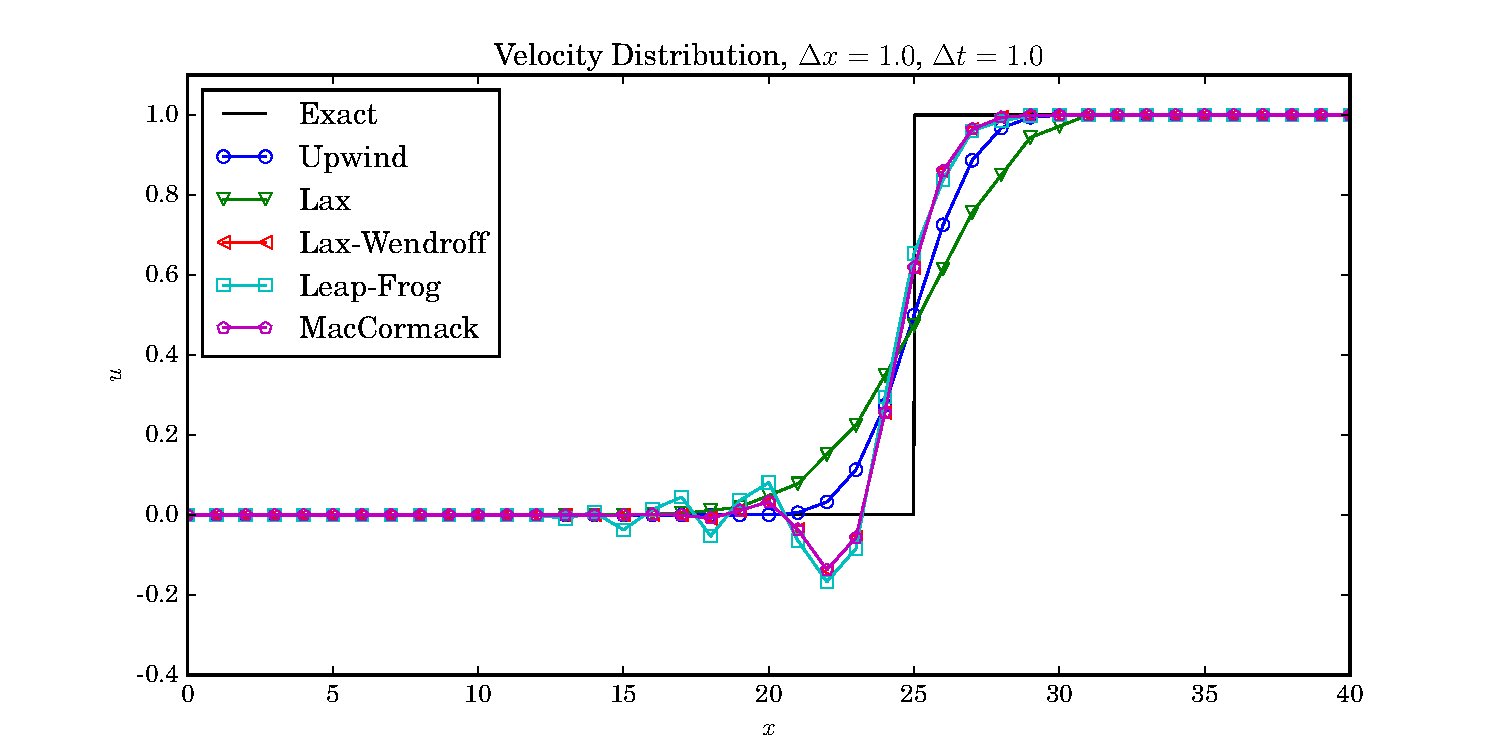
\includegraphics[width = 0.95\textwidth]{./Figures/q1_1}
    \caption{Velocity Distribution for $\Delta t = 1.0$}
    \label{fig:q11}
\end{figure}
\begin{figure}[!h]
    \centering
    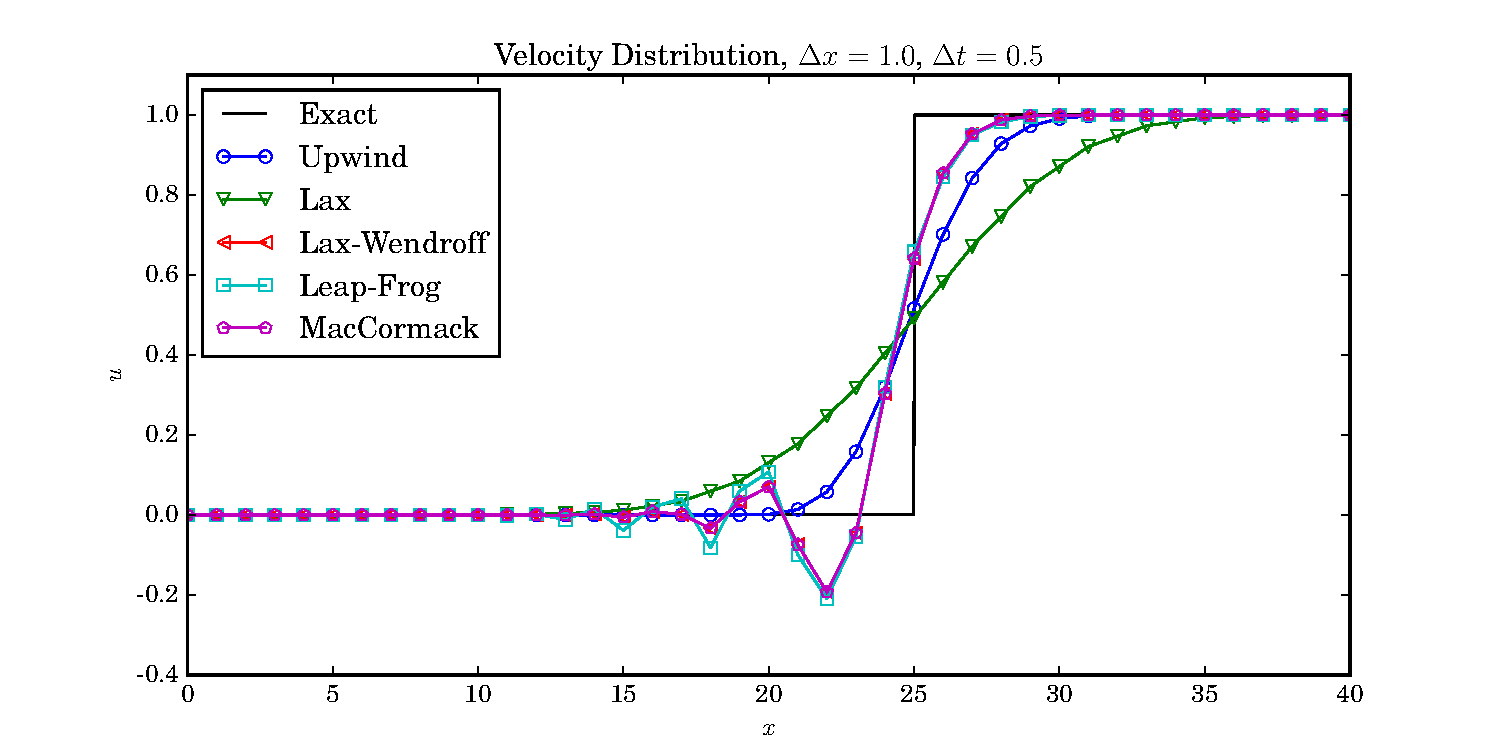
\includegraphics[width = 0.95\textwidth]{./Figures/q1_2}
    \caption{Velocity Distribution for $\Delta t = 0.5$}
    \label{fig:q12}
\end{figure}


\newpage
\section*{Question 2}

The Upwind and MacCormack schemes have been used for the grid study.
The CFL number is kept constant at $CFL = 0.5$, therefore, the time-step is decreased proportionally to the spacing.
Figure \ref{fig:q2} shows the solutions for different grid sizes.
As the grid is refined, the numerical solution approches the exact one. 
\begin{figure}[!h]
    \centering
    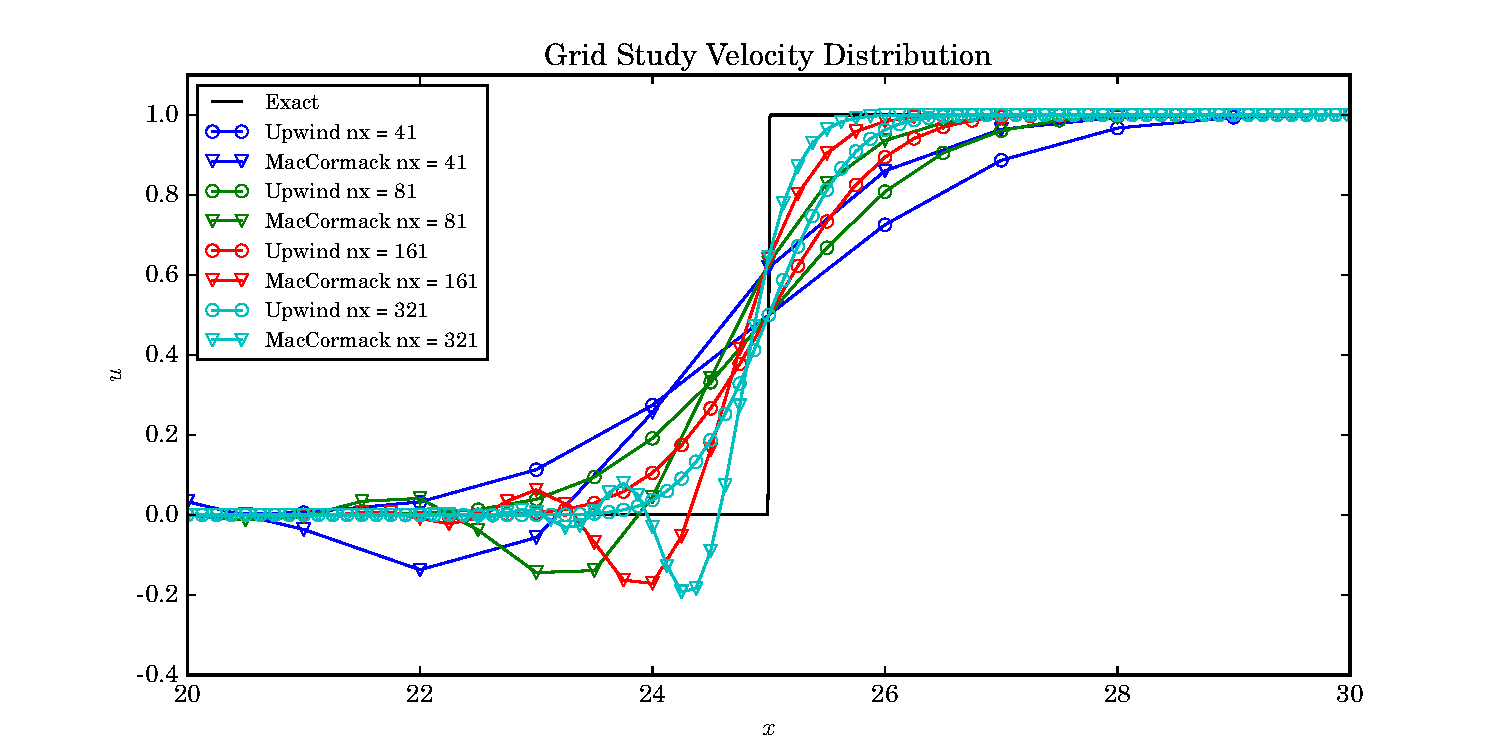
\includegraphics[width = 0.95\textwidth]{./Figures/q2}
    \caption{Grid Study with CFL = 0.5}
    \label{fig:q2}
\end{figure}

\newpage
\section*{Question 3}

To check the order of accuracy, the number of points is doubled from 41 points to 40561 points.
The CFL is kept constant to keep the algorithm stable so the time step is reduced by half every time.

It can be seen in Figure \ref{fig:q3} that the error reduces as the number of points increases.
The slope of each scheme is related to the order of accuracy of the scheme. 
Therefore, it is possible to deduce that the Upwind and Lax schemes are first order accurate, while the others are second order.

\begin{figure}[!h]
    \centering
    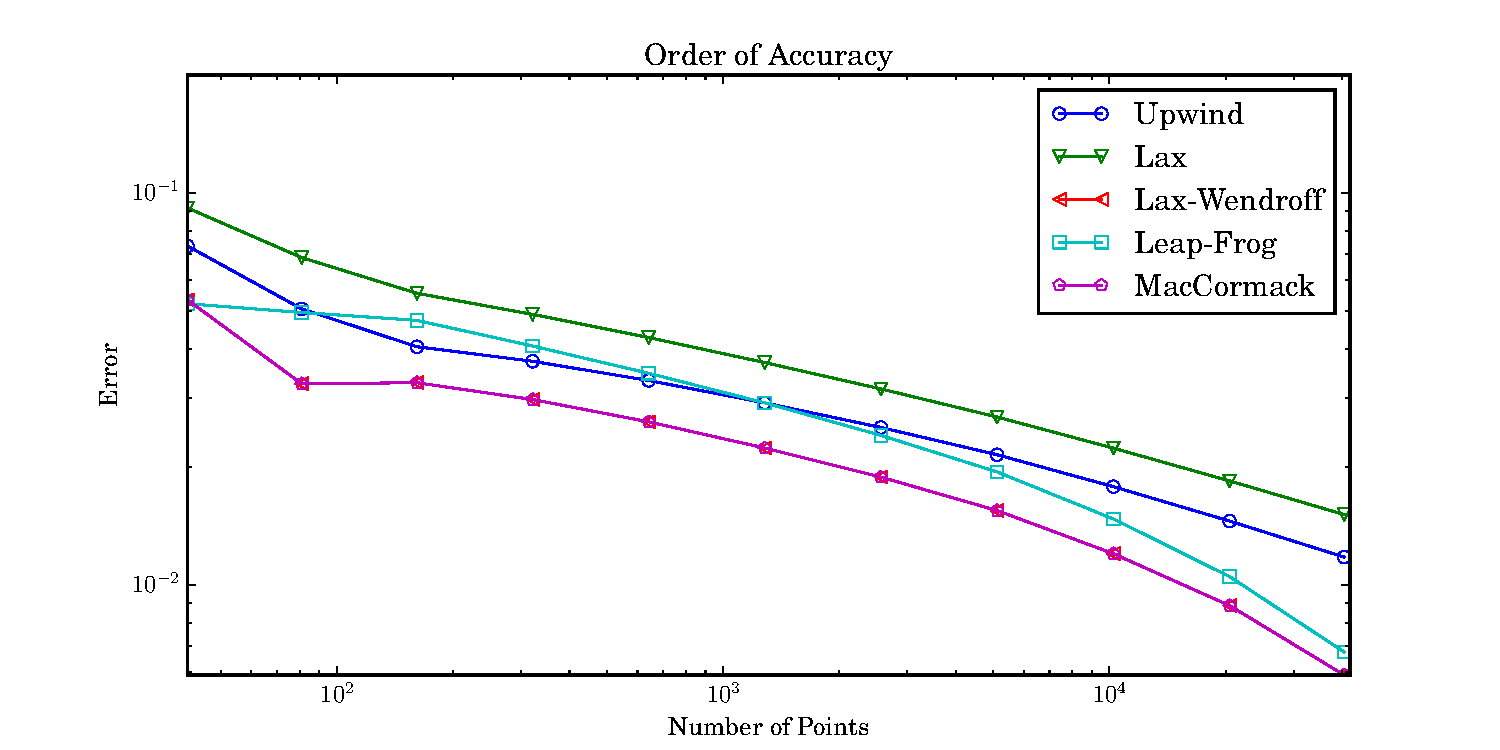
\includegraphics[width = 0.95\textwidth]{./Figures/q3}
    \caption{Order of Accuracy}
    \label{fig:q3}
\end{figure}

\newpage
\section*{Question 4}

The stability condition is derived for both Lax and Lax-Wendroff in the following pages.
A CFL of 1 is found to be the upper bound for a stable scheme in both cases.
Figure \ref{fig:q41} and \ref{fig:q42} show that the error starts increasing as soon as the CFL goes above 1.
The gain in error is small enough to get a converged solution since there are only 10 iterations.
\begin{figure}[!h]
    \centering
    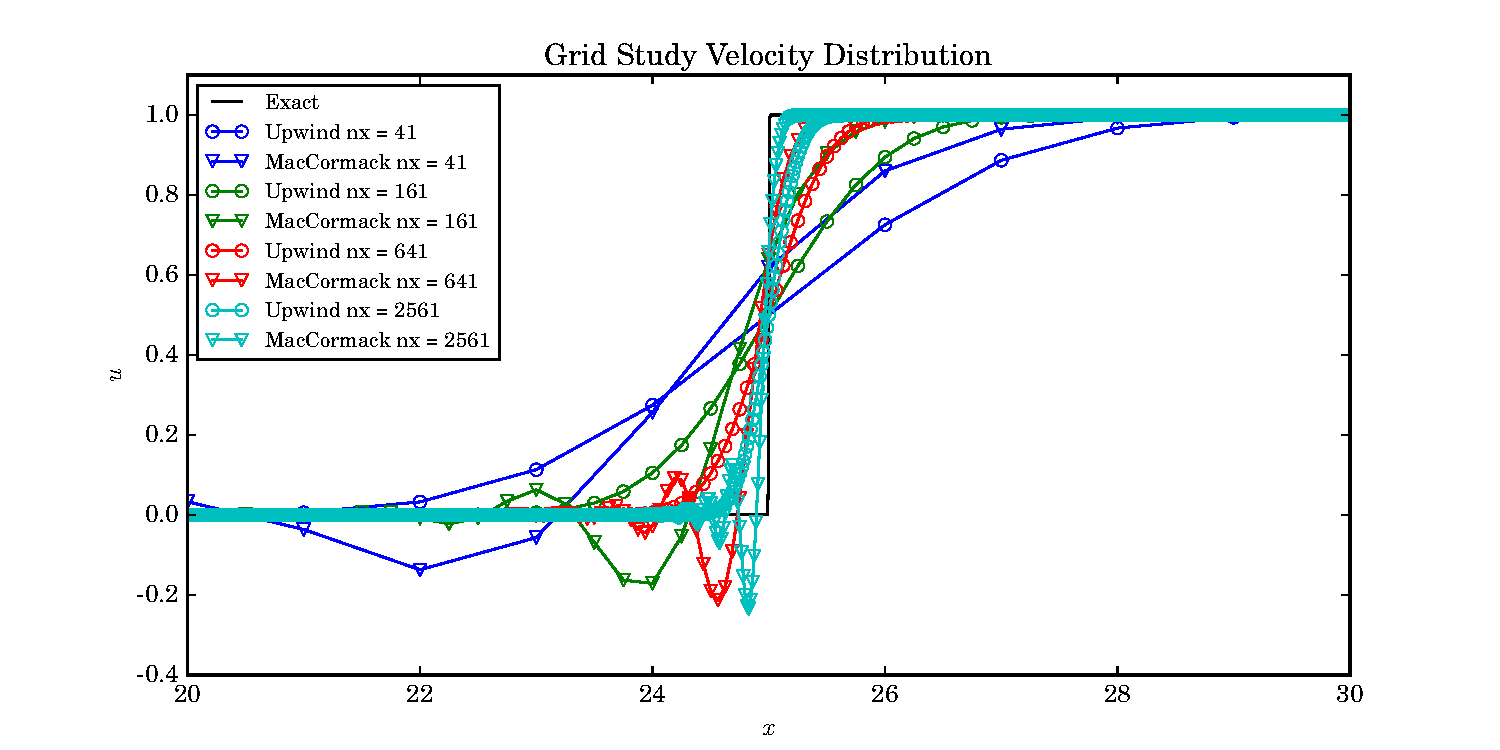
\includegraphics[width = 0.95\textwidth]{./Figures/q4_1}
    \caption{Stability Condition for Lax}
    \label{fig:q41}
\end{figure}
\begin{figure}[!h]
    \centering
    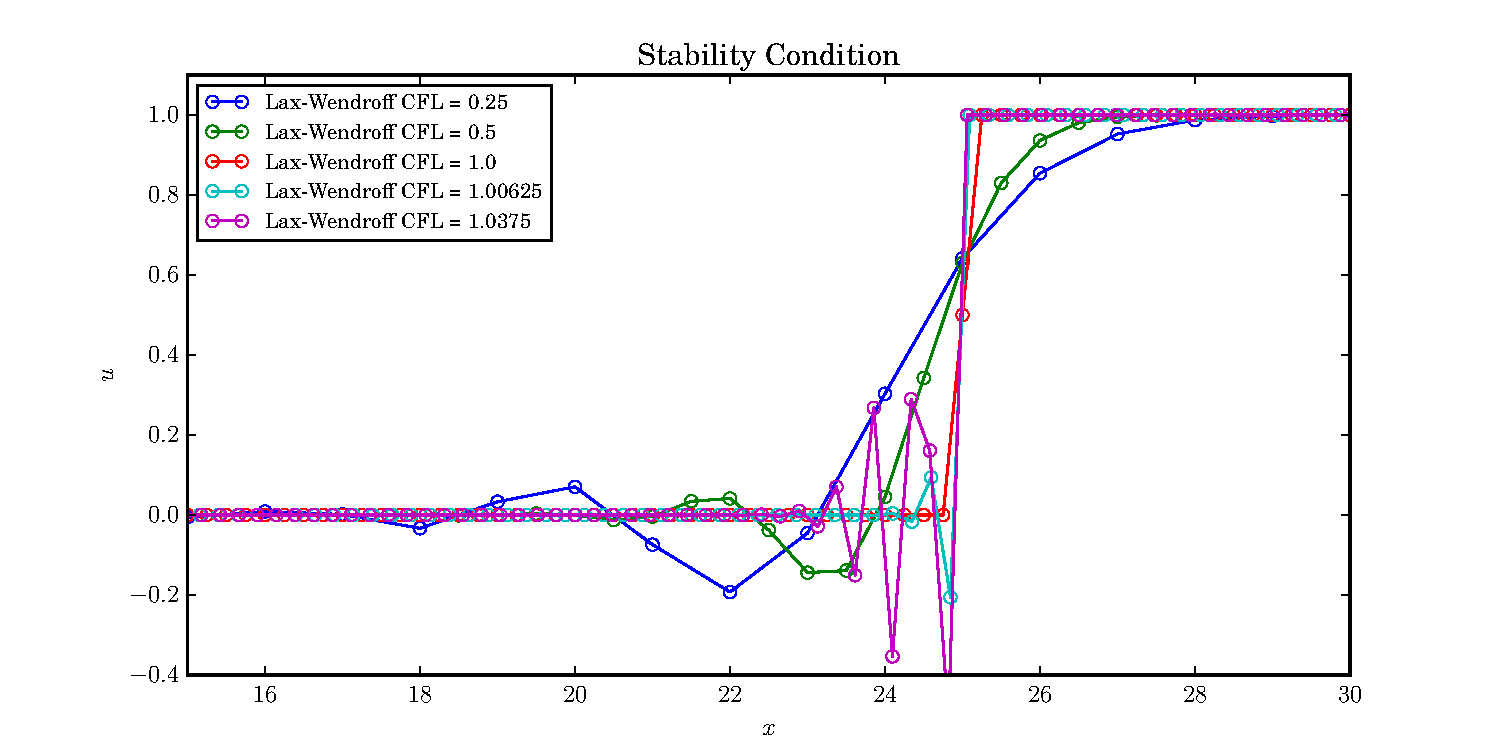
\includegraphics[width = 0.95\textwidth]{./Figures/q4_2}
    \caption{Stability Condition for Lax-Wendroff}
    \label{fig:q42}
\end{figure}

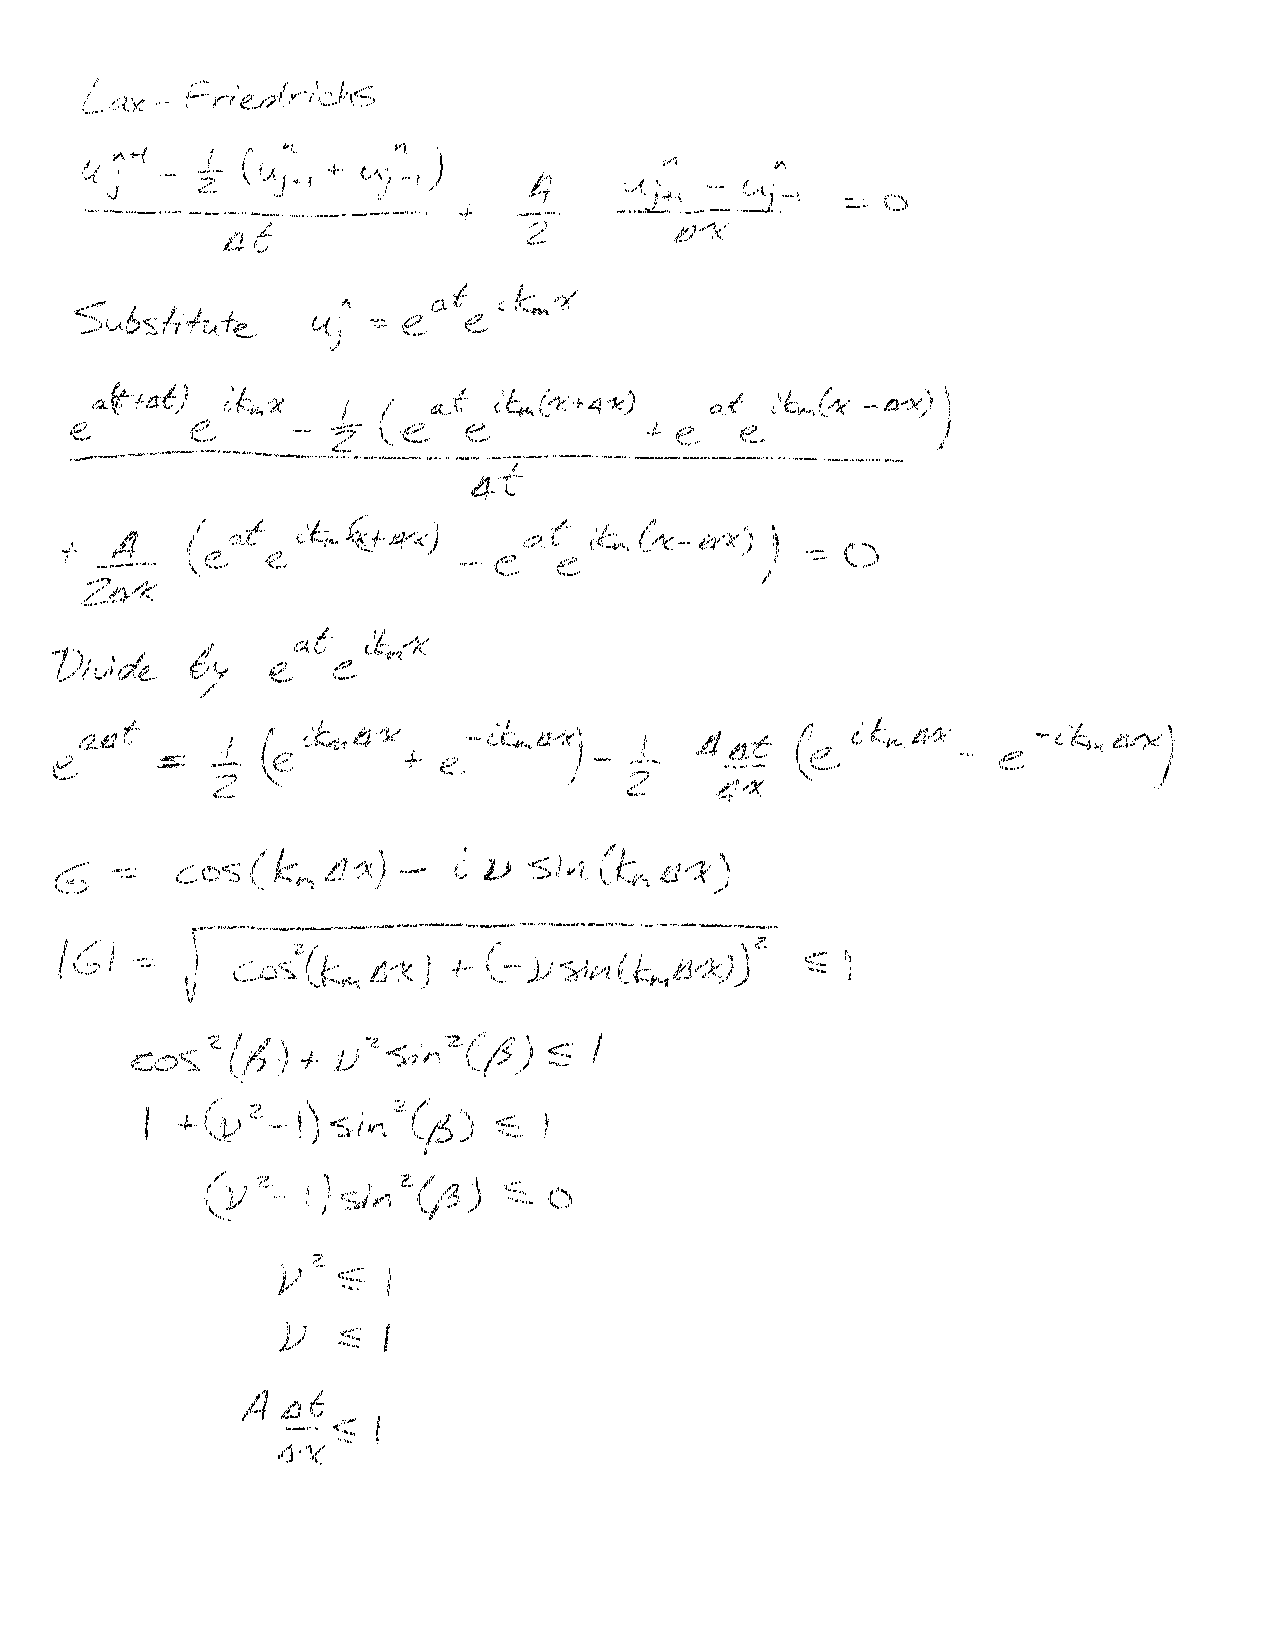
\includepdf[pages={1-2}]{./Figures/derivations.PDF}

\section*{Question 5}

Consistency of Upwind derived in later page.

\section*{Codes}

All codes are available on my GitHub:

\url{https://github.com/dougshidong/mech539/tree/master/a1}

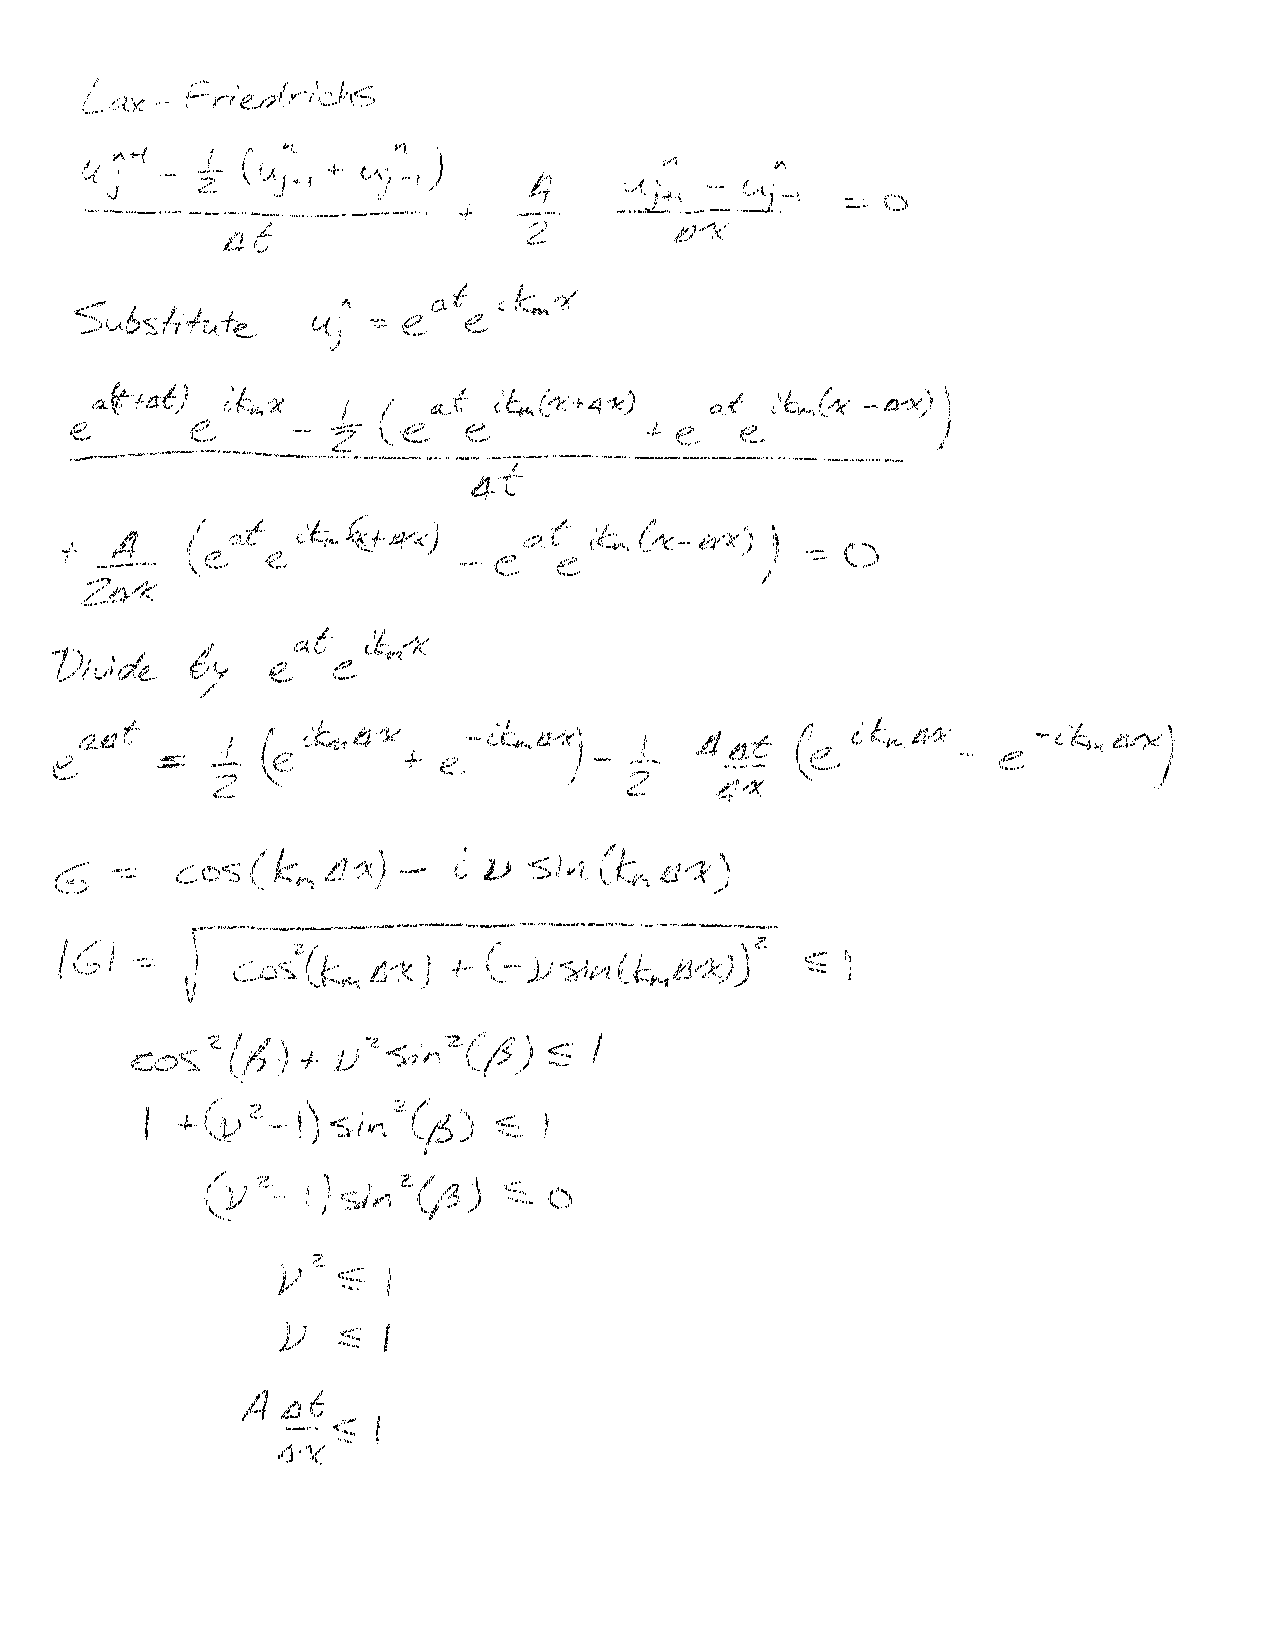
\includepdf[pages={1-2}]{./Figures/derivations.PDF}
\end{document}
